\documentclass[border=8pt, multi, tikz]{standalone}
%\usepackage{blocks}
\usepackage{import}
\subimport{layers/}{init}
\usetikzlibrary{positioning}
\usetikzlibrary{3d} %for including external image 


\def\ConvColor{rgb:yellow,5;red,2.5;white,5}
\def\ConvReluColor{rgb:yellow,5;red,5;white,5}
\def\PoolColor{rgb:red,1;black,0.3}
\def\UnpoolColor{rgb:blue,2;green,1;black,0.3}
\def\ConcatColor{rgb:blue,5;red,2.5;white,5}
\def\FcReluColor{rgb:blue,5;red,5;white,4}
\def\SoftmaxColor{rgb:magenta,5;black,7}
\def\noise{rgb:red,0.5;green,5;black,6}


\newcommand{\copymidarrow}{\tikz \draw[-Stealth,line width =0.8mm,draw={rgb:blue,4;red,1;green,1;black,3}] (-0.3,0) -- ++(0.3,0);}

\begin{document}
\begin{tikzpicture}
\tikzstyle{connection}=[ultra thick,every node/.style={sloped,allow upside down},draw=\edgecolor,opacity=0.7]
\tikzstyle{copyconnection}=[ultra thick,every node/.style={sloped,allow upside down},draw={rgb:blue,4;red,1;green,1;black,3},opacity=0.7]

%%%%%%%%%%%%%%%%%%%%%%%%%%%%%%%%%%%%%%%%%%%%%%%%%%%%%%%%%%%%%%%%%%%%
% training set
%%%%%%%%%%%%%%%%%%%%%%%%%%%%%%%%%%%%%%%%%%%%%%%%%%%%%%%%%%%%%%%%%%%%

\node at (18,5.75,0) {\large{\textbf{Training set (Real images)}}};

\node[canvas is zy plane at x=0] (l1) at (22,12,1)  {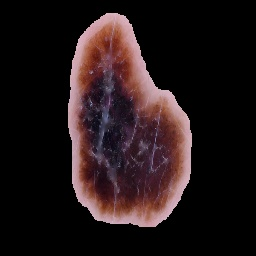
\includegraphics[width=8cm,height=8cm]{l1.jpg} };
\node[canvas is zy plane at x=0] (l2) at (17,12,1) {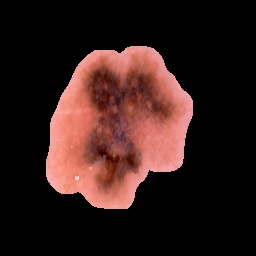
\includegraphics[width=8cm,height=8cm]{l2.jpg} };
\node[canvas is zy plane at x=0] (l2) at (18,12,1) {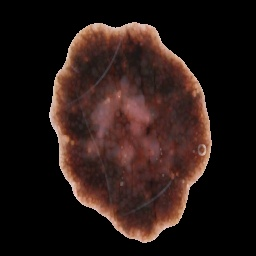
\includegraphics[width=8cm,height=8cm]{lesion.jpg} };
\node[canvas is zy plane at x=0] (l3) at (19,12,1) {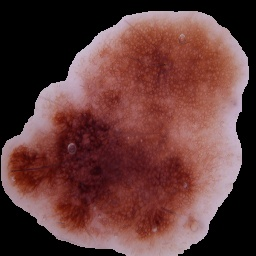
\includegraphics[width=8cm,height=8cm]{l3.jpg} };
\node[canvas is zy plane at x=0] (l4) at (20,12,1) {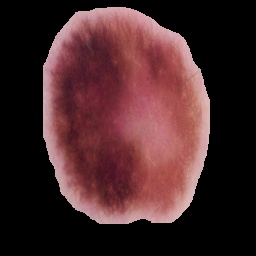
\includegraphics[width=8cm,height=8cm]{l4.jpg} };
\node[canvas is zy plane at x=0] (l5) at (21,12,1) {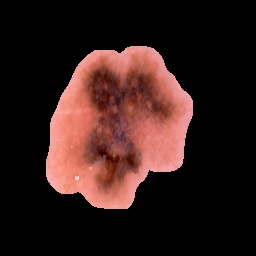
\includegraphics[width=8cm,height=8cm]{l2.jpg} };
% fake conv
\pic[shift={(22,10,0)}] at (0,0,0) {RightBandedBox={name=fc,%
      fill=\ConvColor,bandfill=\ConvReluColo,%
        height=2,width={2},depth=2}};
\node[canvas is zy plane at x=0] (l6) at (23,12,1) {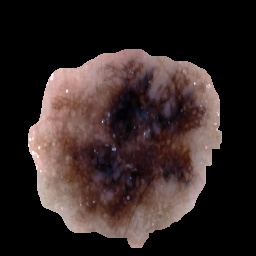
\includegraphics[width=8cm,height=8cm]{l5.jpg} };



%%%%%%%%%%%%%%%%%%%%%%%%%%%%%%%%%%%%%%%%%%%%%%%%%%%%%%%%%%%%%%%%%%%%
% Generator
%%%%%%%%%%%%%%%%%%%%%%%%%%%%%%%%%%%%%%%%%%%%%%%%%%%%%%%%%%%%%%%%%%%%

\node at (10,-7,0) {\Large{\textbf{Generator}}};

% noise
\pic[shift={(0,0,0)}]  at (0,0,0) {RightBandedBox={name=Rn,%
        caption= Random noise ,fill=\noise,bandfill=\noise,%
        height=2 ,width=2,depth=40}};
% conve1
\pic[shift={(2,0,0)}] at (Rn-east) {RightBandedBox={name=c1,%
        xlabel={{"256","256"}}, zlabel=4, caption=deconv1,fill=\ConvColor,bandfill=\ConvReluColor,%
        height=10,width={8},depth=10}};

% conve2
\pic[shift={(1.5,0,0)}] at (c1-east) {RightBandedBox={name=c2,%
        xlabel={{"128","128"}}, zlabel=8, caption=deconv2,fill=\ConvColor,bandfill=\ConvReluColor,%
        height=14,width={7},depth=14}};


% conve3
\pic[shift={(1.5,0,0)}] at (c2-east) {RightBandedBox={name=c3,%
        xlabel={{"64","64"}}, zlabel=16, caption=deconv3,fill=\ConvColor,bandfill=\ConvReluColor,%
        height=16,width={6},depth=16}};

% conve4
\pic[shift={(1.5,0,0)}] at (c3-east) {RightBandedBox={name=c4,%
        xlabel={{"32","32"}}, zlabel=32, caption=deconv4,fill=\ConvColor,bandfill=\ConvReluColor,%
        height=22,width={5},depth=22}};
% conve5
\pic[shift={(1.5,0,0)}] at (c4-east) {RightBandedBox={name=c5,%
        xlabel={{"16","16"}}, zlabel=64, caption=deconv5,fill=\ConvColor,bandfill=\ConvReluColor,%
        height=28,width={4},depth=28}};

% conve6
\pic[shift={(1.5,0,0)}] at (c5-east) {RightBandedBox={name=c6,%
        xlabel={{"8","8"}}, zlabel=128, caption=deconv6,fill=\ConvColor,bandfill=\ConvReluColor,%
        height=34,width={3},depth=34}};

% conve7
\pic[shift={(1.5,0,0)}] at (c6-east) {RightBandedBox={name=c7,%
        xlabel={{"3","3"}}, zlabel=256, caption=deconv7,fill=\ConvColor,bandfill=\ConvReluColor,%
        height=38,width={2},depth=38}};

%leasion
\node[canvas is zy plane at x=0] (l7) at (20.5,0,0) {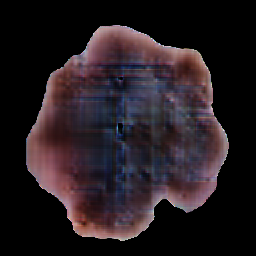
\includegraphics[width=8cm,height=8cm]{Generated.png} };

%%%%%%%%%%%%%%%%%%%%%%%%%%%%%%%%% arrows
\draw [connection]  (Rn-east)        -- node {\copymidarrow} (c1-west);
\draw [connection]  (c1-east)        -- node {\copymidarrow} (c2-west);
\draw [connection]  (c2-east)        -- node {\copymidarrow} (c3-west);
\draw [connection]  (c3-east)        -- node {\copymidarrow} (c4-west);
\draw [connection]  (c4-east)        -- node {\copymidarrow} (c5-west);
\draw [connection]  (c5-east)        -- node {\copymidarrow} (c6-west);
\draw [connection]  (c6-east)        -- node {\copymidarrow} (c7-west);

\node (fake) at (21.5, -5,1) {\large{\textbf{Fake image}}};
% \node (fake) at (22.5, 6.16,1) {\large{\textbf{Real images}}};

%%%%%%%%%%%%%%%%%%%%%%%%%%%%%%%%%%%%%%%%%%%%%%%%%%%%%%%%%%%%%%%%%%%%
% Discriminator
%%%%%%%%%%%%%%%%%%%%%%%%%%%%%%%%%%%%%%%%%%%%%%%%%%%%%%%%%%%%%%%%%%%%

\node at (33,-6,0) {\Large{\textbf{Discriminator}}};

% noise
\pic[shift={(8,-2,0)}] at (c7-north) {RightBandedBox={name=Gn,%
        xlabel={{"3","3"}}, zlabel=256, caption=Gaussian noise,fill=\ConvColor,bandfill=\ConvReluColor,%
        height=38,width={2},depth=38}};
% arrows
\draw [connection]  (c7-east)        -- node {\copymidarrow} (Gn-west);
\draw [connection]  (fc-east)        -- node {\copymidarrow} (Gn-west);

% conve1
\pic[shift={(1.5,0,0)}] at (Gn-east) {RightBandedBox={name=c1,%
        xlabel={{"3","3"}}, zlabel=256, caption=Conv1,fill=\ConvColor,bandfill=\ConvReluColor,%
        height=34,width={3},depth=34}};

% pool 1
\pic[shift={(0,0,0)}] at (c1-east) {Box={name=p1,%
         fill=\PoolColor,opacity=0.5,height=28,width=1,depth=28}};

% conve2
\pic[shift={(1.5,0,0)}] at (p1-east) {RightBandedBox={name=c2,%
        xlabel={{"16","16"}}, zlabel=128, caption=Conv2,fill=\ConvColor,bandfill=\ConvReluColor,%
        height=28,width={4},depth=28}};

% pool 2
\pic[shift={(0,0,0)}] at (c2-east) {Box={name=p2,%
         fill=\PoolColor,opacity=0.5,height=22,width=1,depth=22}};

% conve3
\pic[shift={(1.5,0,0)}] at (p2-east) {RightBandedBox={name=c3,%
        xlabel={{"32","32"}}, zlabel=64, caption=Conv3,fill=\ConvColor,bandfill=\ConvReluColor,%
        height=22,width={5},depth=22}};


% pool 3
\pic[shift={(0,0,0)}] at (c3-east) {Box={name=p3,%
         fill=\PoolColor,opacity=0.5,height=16,width=1,depth=16}};
         
% conve4
\pic[shift={(1.5,0,0)}] at (p3-east) {RightBandedBox={name=c4,%
        xlabel={{"64","64"}}, zlabel=32, caption=Conv4,fill=\ConvColor,bandfill=\ConvReluColor,%
        height=16,width={6},depth=16}};

% pool 4
\pic[shift={(0,0,0)}] at (c4-east) {Box={name=p4,%
         fill=\PoolColor,opacity=0.5,height=12,width=1,depth=12}};
         
% conve5
\pic[shift={(1.5,0,0)}] at (p4-east) {RightBandedBox={name=c5,%
        xlabel={{"128","128"}}, zlabel=16, caption=Conv5,fill=\ConvColor,bandfill=\ConvReluColor,%
        height=12,width={4},depth=12}};

% pool 5
\pic[shift={(0,0,0)}] at (c5-east) {Box={name=p5,%
         fill=\PoolColor,opacity=0.5,height=8,width=1,depth=8}};

         
% conve6
\pic[shift={(1.5,0,0)}] at (p5-east) {RightBandedBox={name=c6,%
        xlabel={{"256","256"}}, zlabel=8, caption=Conv6,fill=\ConvColor,bandfill=\ConvReluColor,%
        height=8,width={3},depth=8}};

% pool 6
\pic[shift={(0,0,0)}] at (c6-east) {Box={name=p5,%
         fill=\PoolColor,opacity=0.5,height=6,width=1,depth=6}};


%%%%%%%%%%%%%%%%%%%%%%%%%%%%%%%%% arrows
\draw [connection]  (Gn-east)        -- node {\copymidarrow} (c1-west);
\draw [connection]  (c1-east)        -- node {\copymidarrow} (c2-west);
\draw [connection]  (c2-east)        -- node {\copymidarrow} (c3-west);
\draw [connection]  (c3-east)        -- node {\copymidarrow} (c4-west);
\draw [connection]  (c4-east)        -- node {\copymidarrow} (c5-west);
\draw [connection]  (c5-east)        -- node {\copymidarrow} (c6-west);


% nodes
\node (real) at (43.5, 3,1) {\large{\textbf{Real}}};
\node (A) at (42, 2,1) {};
\node (fake) at (43.5, 1,1) {\large{\textbf{Fake}}};

% arrows
\draw[->, to path={-| (\tikztotarget)}]
  (A) edge (real) (A) edge (fake) ;


\end{tikzpicture}
\end{document}